\documentclass{beamer}
\usepackage[utf8]{inputenc}
\usepackage[T1]{fontenc}
\usepackage{mathabx}
\usepackage{mathpazo}
\usepackage{eulervm}
\usepackage{natbib}
\usepackage{enumerate}
\usepackage{mathrsfs}

\usetheme{Madrid}
\usefonttheme{structurebold}
\usecolortheme{dove}
\title{VE401 RC Week7}
\author{Wang Yangyang}
\date{2022 Spring}
\institute{UM-SJTU JI}
\setbeamersize{text margin left = 20pt, text margin right = 20pt}

\AtEndDocument{\begin{frame}{End}

                  Credit to Zhanpeng Zhou (TA of SP21)
                  
                  Credit to Fan Zhang (TA of SU21)
                  
                  Credit to Liying Han (TA of SP21)
                  
                  Credit to Zhenghao Gu (TA of SP20)
               \end{frame}}
                
\definecolor{antiquefuchsia}{rgb}{0.57, 0.36, 0.51}
\newcommand{\bb}[1]{\textcolor{antiquefuchsia}{\textbf{\textit{#1}}}}

\begin{document}
\maketitle

\begin{frame}
\frametitle{Outline}
\tableofcontents
\end{frame}

%\AtBeginSection[ ]
%{
%\begin{frame}{Outline for \secname}
%	\tableofcontents[currentsection, hideothersubsections, %sectionstyle=show/show]
%\end{frame}
%}

\AtBeginSubsection[]{
  \frame<beamer>{ 
    \frametitle{Outline}   
    \tableofcontents[currentsection,currentsubsection] 
  }
}

\section{Hypothesis Tests}
\subsection{Fisher's Null Hypothesis Test}
\begin{frame}{Null Hypotheses}
\bb{Null hypotheses} take one of three forms:
$$
\begin{aligned}
&H_{0}: \theta=\theta_{0} \\
&H_{0}: \theta \leq \theta_{0} \\
&H_{0}: \theta \geq \theta_{0}
\end{aligned}
$$
Our goal is to reject the null hypothesis $H_{0}$.

We either
\begin{itemize}
\item fail to reject $H_{0}$ or
\item reject $H_{0}$ at the [\bb{p-value}] level of significance.
\end{itemize}

\end{frame}

\begin{frame}{One-Tailed Test}
\begin{enumerate}
\item Take a random sample of size $n$ and find the value for the estimator $\widehat{\theta}$. Set One-tailed test is the test of a hypothesis of the form
$$
H_{0}: \theta \leq \theta_{0}
$$
or
$$
H_{0}: \theta \geq \theta_{0}
$$
\item Suppose the hypothesis is $H_{0}: \theta \leq \theta_{0}$. Next we calculate the significance or $P$-value of the test, which is the probability of obtaining the measured value of $\widehat{\theta}$ or a larger result if $\theta=\theta_{0}$,

e.g., for $H_{0}: \mu \leq 26$, the $P$-value is
$$
P[\widebar{X} \geq \widebar{x} \mid \mu=26]
$$
\end{enumerate}
\end{frame}

\begin{frame}{One-Tailed Test}
After calculation based on data, we have upper bound of the probability of obtaining the measured value of $\widehat{\theta}$ or a larger result if $H_{0}$ is true, denoted as $P\left[D \mid H_{0}\right]$, and
$$
P\left[D \mid H_{0}\right] \leq P \text {-value }
$$
\begin{center}
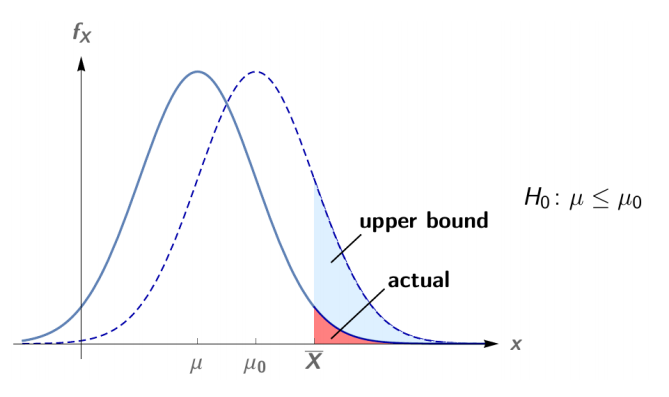
\includegraphics[scale=0.5]{1.png}
\end{center}
\end{frame}

\begin{frame}{Two-Tailed Test}
\begin{enumerate}
\item Take a random sample of size $n$ and find the value for the estimator $\widehat{\theta}$. Set One-tailed test is the test of a hypothesis of the form
$$
H_{0}: \theta=\theta_{0}
$$
\item Next we calculate the significance or $P$-value of the test, which is the probability of obtaining the measured value of $\widehat{\theta}$ or a larger result if $\theta=\theta_{0}$. e.g., for $H_{0}: \mu=40$, find
$$
P[\widebar{X} \geq \widebar{x} \mid \mu=40] \quad \text { or } \quad P[\widebar{X} \leq \widebar{x} \mid \mu=40]
$$
based on different situation.
\item After calculation based on data, we need to double the result to get $P$-value. Then reject $H_{0}$ if $P$-value is small.
\end{enumerate}
\end{frame}

\subsection{Neyman-Pearson Decision Theory}
\begin{frame}{Two Types of Error}
Given a choice between \bb{null hypotheses} $H_{0}$ and \bb{alternative hypotheses} $H_{1}$, there are 4 possible outcomes of the decision-making:
\begin{enumerate}
\item We reject $H_{0}$ (accept $H_{1}$) when $H_{0}$ is false.
\item We reject $H_{0}$ (accept $H_{1}$) even though $H_{0}$ is true (\bb{Type I error}).
\item We fail to reject $H_{0}$ even though $H_{1}$ is true (\bb{Type II error}).
\item We fail to reject $H_{0}$ when $H_{0}$ is true.
\end{enumerate}

$$
\begin{aligned}
\alpha &:=P[\text { Type I error }]=P\left[\text { reject } H_{0} \mid H_{0} \text { true }\right] \\
&=P\left[\text { accept } H_{1} \mid H_{0} \text { true }\right]
\end{aligned}
$$

$$
\begin{aligned}
\beta &:=P[\text { Type II error }]=P\left[\text { fail to reject } H_{0} \mid H_{1} \text { true }\right] \\
&=P\left[\text { accept } H_{0} \mid H_{1} \text { true }\right]
\end{aligned}
$$

$$
 \begin{aligned}\text { Power }
&:=1-\beta=P\left[\text { reject } H_{0} \mid H_{1} \text { true }\right] \\
&=P\left[\text { accept } H_{1} \mid H_{1} \text { true }\right]
\end{aligned}
$$

\end{frame}

\begin{frame}{Procedure}
\begin{enumerate}
\item Set up a \bb{null hypothesis} $H_{0}$ and an \bb{alternative hypothesis} $H_{1}$.
\item Determine a desirable $\alpha$ and $\beta$.
\item Use $\alpha$ and $\beta$ to determine the appropriate \bb{sample size} $n$.
\item Use $\alpha$ and $n$ to determine the \bb{critical region}.
\item Obtain sample statistics, and reject $H_{0}$ at significance level $\alpha$ and accept $H_{1}$ if the test statistic falls into critical region. Otherwise, accept $H_{0}$.
\end{enumerate}
Step 1 and 2 are significant before obtaining data.

Step 3 and 4 requires clear calculation and analysis.

The sample size, the critical region must be fixed before data are obtained.
\end{frame}

\begin{frame}{$\alpha$ and the Critical Region}
\begin{block}{Definition}
\begin{itemize}
\item If $H_{0}$ is true, then the probability of the test statistic's values falling into the \bb{critical region} is not more than $\alpha$.
\item If the value of the test statistic falls into the critical region, then we reject $H_{0}$.
\end{itemize}
\end{block}
\begin{block}{Example}
Suppose the sample mean $\widebar{X}$ follows a normal distribution with unknown mean $\mu$ and known variance $\sigma^{2}$, with $H_{0}: \mu=\mu_{0}$.
$$
Z=\frac{\widebar{X}-\mu_{0}}{\sigma / \sqrt{n}}
$$
\end{block}


\end{frame}

\begin{frame}{$\alpha$ and the Critical Region}
\begin{block}{Example}
$Z$ follows a standard normal distribution. The critical region is determined by
$$
\frac{\left|\widebar{X}-\mu_{0}\right|}{\sigma / \sqrt{n}}>z_{\alpha / 2}
$$
or
$$
\widebar{x} \neq \mu_{0} \pm z_{\alpha / 2} \frac{\sigma}{\sqrt{n}}
$$
\end{block}
\begin{block}{Remarks}
\begin{enumerate}
\item We only care about the probability of committing an error if $H_{0}$ is falsely rejected.
\item Only $H_{0}$ plays a role in the calculation of the critical region. $H_{1}$ does not enter into the discussion.
\end{enumerate}
\end{block}
\end{frame}

\begin{frame}{$\beta$ and the Sample Size}
The second type of error concerns failing to reject $H_{0}$ even though $H_{1}$ is true. Suppose
$
H_{0}: \mu=\mu_{0}, \quad H_{1}:\left|\mu-\mu_{0}\right| \geq \delta_{0}
$.

Suppose the true value of mean is $\mu=\mu_{0}+\delta, \delta>0$. The test statistic
$$
Z=\frac{\widebar{X}-\mu_{0}}{\sigma / \sqrt{n}}
\sim\text{N}(\delta \sqrt{n} / \sigma,1)$$

Supposing that $\alpha$ has been fixed, we will fail to reject $H_{0}$ if
$$
-z_{\alpha / 2} \leq Z \leq z_{\alpha / 2}
$$
\begin{center}
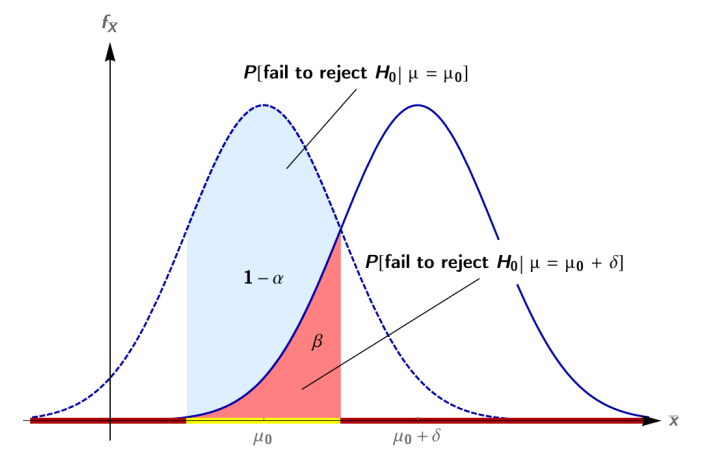
\includegraphics[scale=0.36]{2.png}
\end{center}
\end{frame}

\begin{frame}{$\beta$ and the Sample Size}
With true mean $\mu=\mu_{0}+\delta$, the test statistic $Z=\frac{\widebar{X}-\mu_{0}}{\sigma / \sqrt{n}} \sim \mathrm{N}(\delta \sqrt{n} / \sigma, 1)$.
$$
\begin{aligned}
P&\left[\text { fail to reject } H_{0} \mid \mu=\mu_{0}+\delta\right] =\frac{1}{\sqrt{2 \pi}} \int_{-z_{\alpha / 2}}^{z_{\alpha / 2}} e^{-(t-\delta \sqrt{n} / \sigma)^{2} / 2} \mathrm{~d} t \\
&=\frac{1}{\sqrt{2 \pi}} \int_{-z_{\alpha / 2}-\delta \sqrt{n} / \sigma}^{z_{\alpha / 2}-\delta \sqrt{n} / \sigma} e^{-t^{2} / 2} \mathrm{~d} t  \approx \frac{1}{\sqrt{2 \pi}} \int_{-\infty}^{z_{\alpha / 2}-\delta \sqrt{n} / \sigma} e^{-t^{2} / 2} \mathrm{~d} t \stackrel{!}{=} \beta,
\end{aligned}
$$
where we set $-z_{\beta}=z_{\alpha / 2}-\delta \sqrt{n} / \sigma$.
$$
n \approx \frac{\left(z_{\alpha / 2}+z_{\beta}\right)^{2} \sigma^{2}}{\delta^{2}}
$$
where $z_{\alpha / 2}$ and $z_{\beta}$ satisfies that
$$
\Phi\left(z_{\alpha / 2}\right)=1-\alpha / 2, \quad \Phi\left(z_{\beta}\right)=1-\beta
$$
\end{frame}

\begin{frame}{$\beta$ and the Sample Size}
\begin{block}{Remarks}
The result applies to \bb{normal} case.
\begin{enumerate}
\item A desired (small) $\beta$ can be attained by choosing an appropriate sample size $n$.
\item Power $=1-\beta$. Generally, we would like the probability of rejecting $H_{0}$ if the alternative hypothesis is true to be high, i.e., Power $=1-\beta$ to be high.
\end{enumerate}
\end{block}
In practice, it may be difficult to perform integral calculations every time to find the probability of failing to reject $H_{0}$ as an integral. For this reason, we can refer to \bb{OC curves} to read $\beta$ directly. Each single curve represents a choice of test parameters $\alpha$ and $n$.
\end{frame}

\begin{frame}{OC Curves}
\begin{itemize}
\item For normal test, calculate
$$
d:=\frac{\left|\mu-\mu_{0}\right|}{\sigma} .
$$
Note. The \bb{abscissa} might change corresponding to the distribution of test.\item Look up in OC curve for sample size $n$.
\end{itemize}
\begin{block}{Remarks}
\begin{itemize}
\item Be careful with the \bb{horizontal axis} for each type of OC curve.
\item For the same distribution, OC curves are different for one-sided or two-sided tests.
\end{itemize}
\end{block}
\end{frame}

\begin{frame}{OC Curves}
\begin{center}
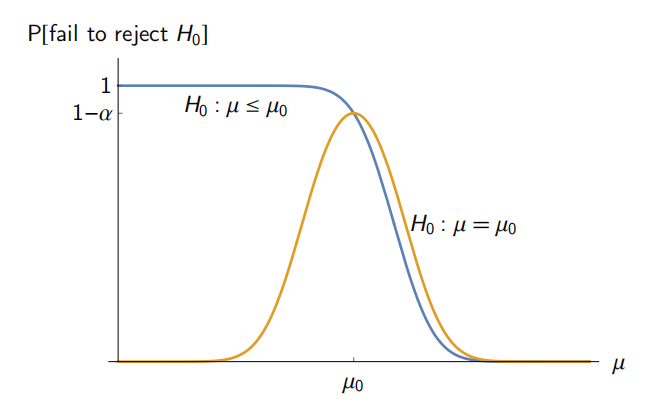
\includegraphics[scale=0.3]{3.png}
\end{center}
\begin{center}
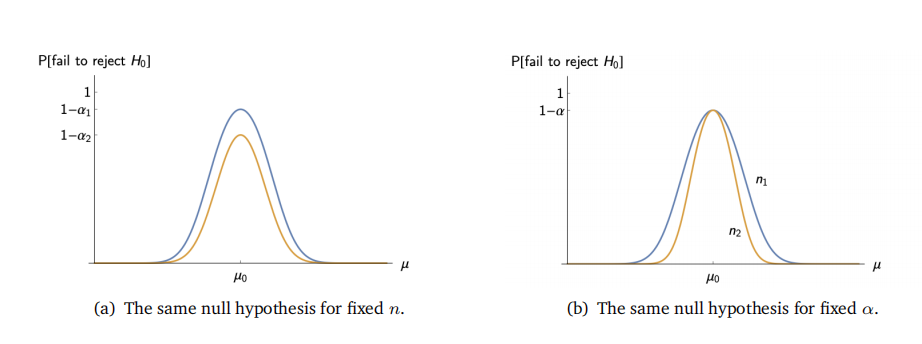
\includegraphics[scale=0.45]{4.png}
\end{center}
\end{frame}

\begin{frame}{OC Curves}
\begin{center}
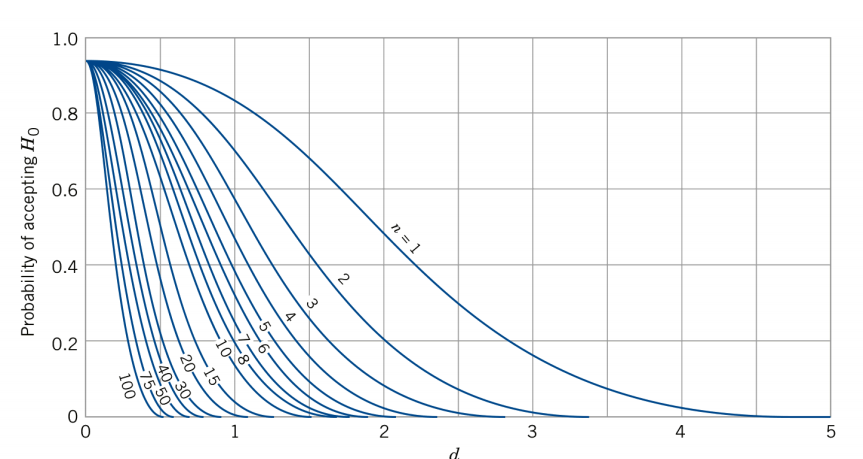
\includegraphics[scale=0.45]{5.png}
\end{center}
\end{frame}

\begin{frame}{Relation between CI and CR}
We have seen that the two-tailed null hypothesis $H_{0}: \mu=\mu_{0}$ is rejected if
$$
\widebar{X} \neq \mu_{0} \pm z_{\alpha / 2} \frac{\sigma}{\sqrt{n}}
$$
This is equivalent to
$$
\mu_{0} \neq \widebar{X} \pm z_{\alpha / 2} \frac{\sigma}{\sqrt{n}}
$$

Suppose we would like to estimate the mean $\mu$ of a sample $X_{1}, \ldots, X_{n}$ of size $n$.
\begin{itemize}
\item \bb{Confidence interval}. Given a sample data with specific values, the $CI$ gives an interval for the unknown mean $\mu$.
\item \bb{Critical region}. Given a null value $\mu_{0}$, the critical region gives an interval for sample mean $\widebar{X}$ before obtaining 
\end{itemize}
The null hypothesis $H_{0}$ is rejected $\Leftrightarrow \widebar{X}$ lies in the critical region $\Leftrightarrow$ null value $\mu_{0}$ lies outside the confidence interval.
\end{frame}

\begin{frame}{Relation between Two Tests}
\begin{enumerate}
\item 
\bb{Neyman-Pearson}: $\widebar{X}$ lies in the critical region for $\alpha$ if and only if the null value $\mu_{0}$ does not lie in a $100(1-\alpha) \%$ two-sided confidence interval for $\mu$.

\bb{Fisher}: $H_{0}$ is rejected at significance level $\alpha$ if and only if the null value $\mu_{0}$ does not lie in a $100(1-\alpha) \%$ two-sided confidence interval for $\mu$.

(This generalizes to one-sided tests and is also true for other distributions.)
\item If the P-value in Fisher's test is no greater than the value of $\alpha$ in Neyman-Pearson's decision process, then $H_{0}$ is rejected and $H_{1}$ accepted. Otherwise, $H_{0}$ is not rejected.
\end{enumerate}
\end{frame}


\subsection{Null Hypothesis Significance Testing (Horrible!)}
\begin{frame}{Procedure}
\begin{enumerate}
\item Two hypotheses, $H_{0}$ and $H_{1}$ are set up, but $H_{1}$ is always the \bb{logical negation} of $\mathrm{H}_{0}$

\item Then either a "hypothesis test" is performed, whereby a \bb{critical region} for given $\alpha$ is defined, the test statistic is evaluated and $H_{0}$ is either rejected or accepted.

Alternatively (and more commonly), the test statistic is evaluated immediately, a $P{\text {-value }}$ is found, and $H_{0}$ is either rejected or accepted based on that value.

\item In either case, there is \bb{no meaningful discussion} of $\beta$, since $H_{1}$ is exactly the negation of $\mathrm{H}_{0}$.
\end{enumerate}
\end{frame}

\begin{frame}{Criticism}
\begin{itemize}
\item A small $P$-value does not guarantee that a large probability that $H_{0}$ is false. Fisher did not intend for a small $P$-value to lead to a clear rejection of $H_{0}$, but only to serve as \bb{evidence against} $H_{0}$ if little else is known.
\item Rejecting $H_{0}$ based on $\alpha=0.05$ or $0.01$ or any other \bb{P-value} is arbitrary.
\item NHST is actually \bb{biased against} failing to reject $\boldsymbol{H}_{0}$. From a Bayesian point of view, it is far too easy to reject $H_{0}$ because $P\left[H_{0}\right]$ does not enter into NHST.
\item A \bb{two-sided test} such as $H_{0}: \theta=\theta_{0}, H_{1}: \theta \neq \theta_{0}$ is meaningless.
\item The \bb{power} ($\beta$) of the test is not properly defined, since $H_{1}$ is just the alternative "not $H_{0}$ " rather than referring to a distinct value $\theta_{1}$.
\end{itemize}
\end{frame}

\section{Single Sample Tests}
\subsection{Single Sample Tests for the Mean and Variance}
\begin{frame}{Test for Mean (Variance Known)}
Let $X_{1}, \ldots, X_{n}$ be a random sample of size $n$ from a \bb{normal} distribution with \bb{unknown} mean $\mu$ and \bb{known} variance $\sigma^{2}$. Let $\mu_{0}$ be a null value of the mean. Then the test statistic is given by
$$
Z=\frac{\widebar{X}-\mu_{0}}{\sigma / \sqrt{n}}
$$
We reject at significance level $\alpha$
\begin{itemize}
\item $H_{0}: \mu=\mu_{0}$ if $|Z|>z_{\alpha / 2}$,
\item $H_{0}: \mu \leq \mu_{0}$ if $Z>z_{\alpha}$,
\item $H_{0}: \mu \geq \mu_{0}$ if $Z<-z_{\alpha}$.
\end{itemize}
\textit{OC curve}. The abscissa is defined by
$$
d=\frac{\left|\mu-\mu_{0}\right|}{\sigma} .
$$
\end{frame}


\begin{frame}{Test for Mean (Variance Unknown)}
Let $X_{1}, \ldots, X_{n}$ be a random sample of size $n$ from a \bb{normal} distribution with \bb{unknown} mean $\mu$ and \bb{unknown} variance $\sigma^{2}$. Let $\mu_{0}$ be a null value of the mean. Then the test statistic is given by
$$
T_{n-1}=\frac{\widebar{X}-\mu_{0}}{S / \sqrt{n}}
$$
We reject at significance level $\alpha$
\begin{itemize}
\item $H_{0}: \mu=\mu_{0}$ if $\left|T_{n-1}\right|>t_{\alpha / 2, n-1}$,
\item $H_{0}: \mu \leq \mu_{0}$ if $T_{n-1}>t_{\alpha, n-1}$,
\item $H_{0}: \mu \geq \mu_{0}$ if $T_{n-1}<-t_{\alpha, n-1}$.
\end{itemize}
\textit{OC curve}. The abscissa is defined by
$$
d=\frac{\left|\mu-\mu_{0}\right|}{\sigma}
$$
\end{frame}

\begin{frame}{Comments on T-test}
\begin{enumerate}
\item The $T$-distribution may be used for $\frac{\widebar{X}-\mu_{0}}{S / \sqrt{n}}$ when a sample is obtained from a normal population.
\item If a sample is obtained from a non-normal population, then for large to medium sample sizes ( $n \geq 25)$ it can be shown that violating the normality assumption does not significantly change $\alpha$ and $\beta$.
\item For small sample sizes, a $T$-test cannot be used and an alternative (non-parametric) test must be employed.
\end{enumerate}
\end{frame}

\begin{frame}{Comments on Abscissa}
Abscissa of OC Curves.
$$
d=\frac{\left|\mu-\mu_{0}\right|}{\sigma}
$$
where $\sigma$ is the unknown standard deviation of the random variable. We have three options:
\begin{enumerate}
\item If available, we can use prior experiments to insert a rough estimate for $\sigma$
\item We can express the difference $\delta=\left|\mu-\mu_{0}\right|$ relative to $\sigma$, e.g., prescribing $d=\delta / \sigma<1$ for a small difference in the mean or $d=\delta / \sigma<2$ for a moderately large difference.
\item We substitute the sample standard deviation $s$ for $\sigma$.
\end{enumerate}
\end{frame}

\begin{frame}{Test for Variance}
Let $X_{1}, \ldots, X_{n}$ be a random sample of size $n$ from a \bb{normal} distribution with \bb{unknown} variance $\sigma^{2}$. Let $\sigma_{0}^{2}$ be a null value of the variance. Then the test statistic is given by
$$
\chi_{n-1}^{2}=\frac{(n-1) S^{2}}{\sigma_{0}^{2}} .
$$
We reject at significance level $\alpha$
\begin{itemize}
\item $H_{0}: \sigma=\sigma_{0}$ if $\chi_{n-1}^{2} \in\left(0, \chi_{1-\alpha / 2, n-1}^{2}\right) \cup\left(\chi_{\alpha / 2, n-1}^{2}, \infty\right)$,
\item $H_{0}: \sigma \leq \sigma_{0}$ if $\chi_{n-1}^{2}>\chi_{\alpha, n-1}^{2}$,
\item $H_{0}: \sigma \geq \sigma_{0}$ if $\chi_{n-1}^{2}<\chi_{1-\alpha, n-1}^{2}$.
\end{itemize}
\textit{OC curve}. The abscissa is defined by
$$
\lambda=\frac{\sigma}{\sigma_{0}}
$$
\end{frame}

\begin{frame}{Comments on Chi-squared Test}
\begin{itemize}
\item If the distribution is non-normal, we cannot use Chi-squared test.
\item ${ }^{* *}$ Normality of the data must first be tested if we do not know the distribution.
\end{itemize}
Abscissa of OC Curves.
$$
\lambda=\frac{\sigma}{\sigma_{0}}
$$
Note that the OC curves for the left- and right-tailed chi-squared distributions are distinct.
\end{frame}

\end{document}